% ----------------------------------------

\subsection{Contextual hypotesis}

% ----------------------------------------

\begin{frame}

\frametitle{Scenario}

We now assume that the binary features of the users cannot be observed and therefore data is considered as \textbf{aggregated}.

Since the features of the users are \textbf{not observable}, the $\alpha$ functions' shape for each class is unknown.

As a result, in our scenario the learner receives all the interactions minus the parameters of the $\alpha$ functions.

\end{frame}

% ----------------------------------------

\subsection{Algorithm}

% ----------------------------------------

\begin{frame}

\frametitle{Solving the problem}

By gathering the aggregated reward for each product we are able to utilize those coarse rewards to generate feedbacks for our \textbf{MABs} and therefore train them on the aggregated interactions for each day.

In particular we exploit \textbf{Gaussian Processes} in conjunction with \textbf{MAB} algorithms such as \textbf{Thompson Sampling} and \textbf{UCB1} to exloit the continuity between the different arms

We instantiate a \textbf{GP-MAB} for each subcampaign and each \textbf{MAB} will have \texttt{n\_budget\_steps} number of arms.

\end{frame}

% ----------------------------------------

\begin{frame}

\frametitle{Algorithms outline}
\framesubtitle{GP TS}

\textbf{GPTS} is a variant of \textbf{TS} implemented using \textbf{Gaussian Processes}:

\begin{itemize}[label={$\circ$}]
	\item For each day $t$, we gather a sample from each arm $a$:
		\begin{displaymath}
			\tilde{\theta_a} \leftarrow \text{ Sample} \left( \mathbb{P}(\mu_a = \theta_a) \right)
		\end{displaymath}
	\item Play arm $a_t$ defined as:
		\begin{displaymath}
			a_t \leftarrow arg\max_{a \in A} \left\{ \tilde{\theta_a} \right\}
		\end{displaymath}
	\item Update the \textbf{Gaussian Process} with the reward obtained.
\end{itemize}

\end{frame}

% ----------------------------------------

\begin{frame}[fragile]

\frametitle{Algorithms outline}
\framesubtitle{GP UCB1}

\textbf{GPUCB1} is a variant of \textbf{UCB1} that takes advantage of the \textbf{Gaussian Processes} confidence interval and models it as the confidence bound; aprat from the arm choice, the learning process is equal to \textbf{GPTS}.

\begin{displaymath}
	a_t \leftarrow arg\max_{a \in A} \left\{ \mu_{t-1} + \delta \sigma_{t-1} \right\}
\end{displaymath}

Code snippet that calculates the \textbf{upper bound}:

\begin{lstlisting}[style=Python, basicstyle=\tiny, numbers=none, xrightmargin=15px]
def estimation(self):
	upper_bounds = (self.means + self.confidence * 1.96 * self.sigmas)
			* self.normalize_factor
	return upper_bounds
\end{lstlisting}

\end{frame}

% ----------------------------------------

\subsection{Results}

% ----------------------------------------

\begin{frame}[plain]

\frametitle{Single run reward and regret}
\framesubtitle{Thompson Sampling and UCB}

\begin{center}
	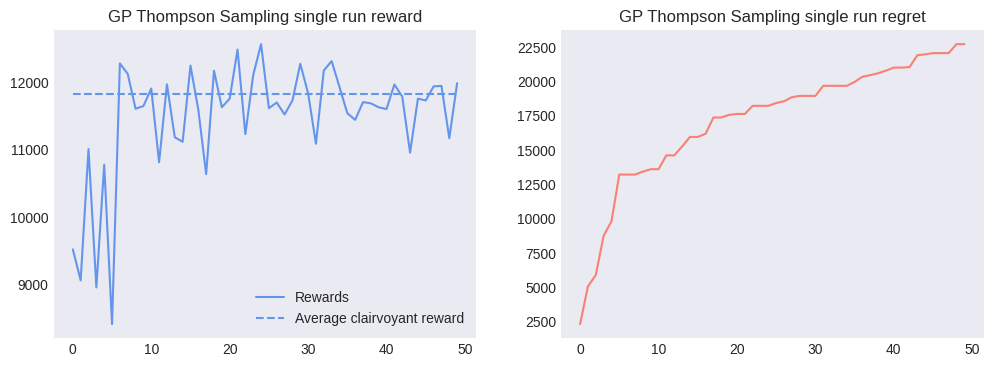
\includegraphics[scale=0.4]{img/Graphs/uncertain_alpha/image1.png}
	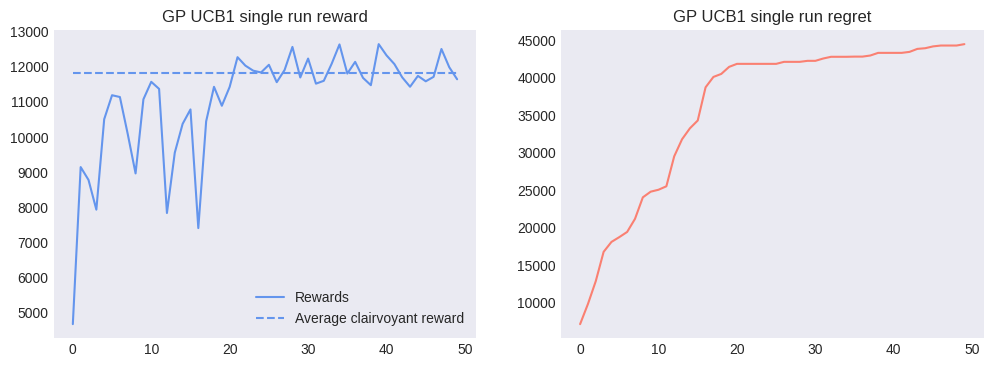
\includegraphics[scale=0.4]{img/Graphs/uncertain_alpha/image2.png}
\end{center}

\end{frame}

% ----------------------------------------

\begin{frame}[plain]

\frametitle{Regret comparison}
\framesubtitle{Thompson Sampling and UCB}

\begin{center}
	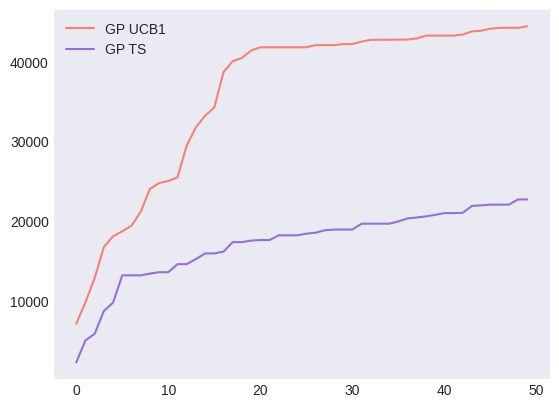
\includegraphics[scale=0.5]{img/Graphs/uncertain_alpha/image3.png}
\end{center}

\scriptsize All tests are done using the \texttt{example\_environment} default values, \textit{population mean} of 1000, \textit{variance} of 10 and 20 \textit{budget steps}.

\end{frame}

% ----------------------------------------

\begin{frame}[plain]

\frametitle{Average regret and reward}
\framesubtitle{Thompson Sampling and UCB}

\begin{center}
	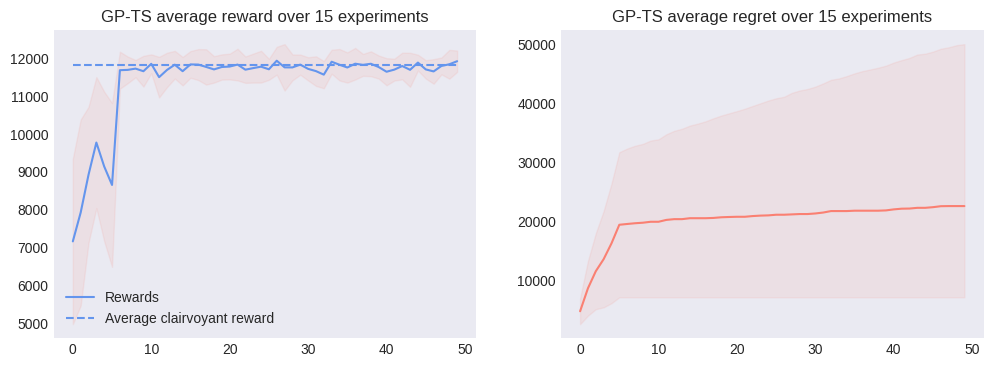
\includegraphics[scale=0.4]{img/Graphs/uncertain_alpha/image4.png}
	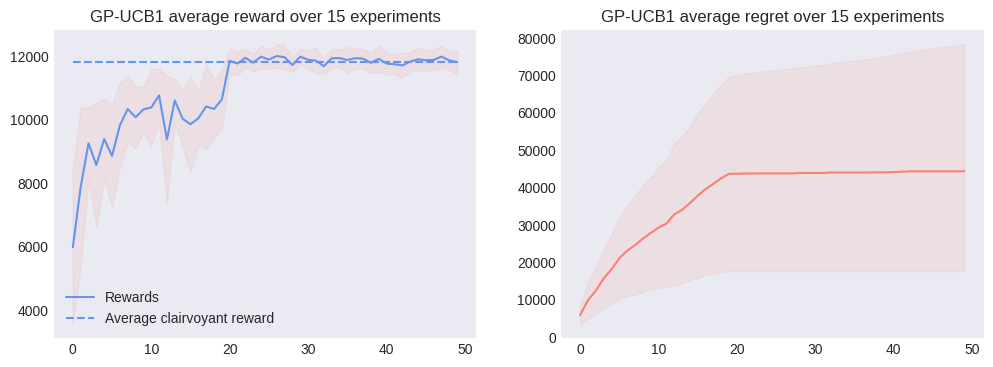
\includegraphics[scale=0.4]{img/Graphs/uncertain_alpha/image5.png}
\end{center}

\end{frame}

% ----------------------------------------

\begin{frame}[plain]

\frametitle{Average regret comparison}
\framesubtitle{Thompson Sampling and UCB}

\begin{center}
	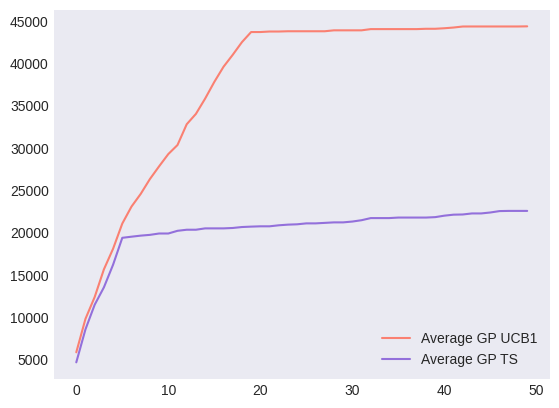
\includegraphics[scale=0.45]{img/Graphs/uncertain_alpha/image6.png}
\end{center}

\begin{displaymath}
	\text{Regret ratio } = \frac{\text{Avg regret}}{\text{Upper bound}} = \frac{31019.40}{?} = ?
\end{displaymath}

\scriptsize Values reference GPTS regret compared to advertising GP regret found at [SLIDE REFERENCE]

\todo{complete}

\end{frame}

% ----------------------------------------

\begin{frame}

\frametitle{Results}

Overall we can observe more instability in the \textbf{TS} algorithm, but a faster convergence w.r.t to the \textbf{UCB} approach.

Both algorithms clearly converge to the optimal solution at different rates while respecting a linear cumulative regret bound.

Average results over 15 runs at time horizon $T = 50$:

\begin{table}
	\begin{tabular}{|c|cc|c|}
	\hline \hline
		\cellcolor{blue!25} & Reward 	& Regret	& Deviation \\
	\cline{2-4}
		\cellcolor{blue!25} & $\mu$		& $\mu$		& $\sigma$	\\
	\hline \hline
		GPTS 				& 11610.53 	& 31024.67	& 440.36 	\\
	\hline
		GPUCB				& 11737.73	& 43686.67	& 349.47	\\
	\hline \hline
	\end{tabular}
\end{table}

\end{frame}

% ----------------------------------------
